\chapter{Experimental Results and Discussion}
\label{ch:results}

This chapter reports the experiments conducted during FYP-I and discusses what they show. It follows the two evidence paths of Chapter \ref{ch:method}. The perception experiments measure detection, counting, and queue estimation on public UA-DETRAC and COCO data. The simulation experiments compare the three signal controllers, static and dynamic ambulance routing, and the green corridor on the synthetic SUMO grid. Every number in this chapter comes from a recorded run whose configuration, seed, and software versions are stored in the project repository, and unfavourable results are reported alongside favourable ones.

\section{Experimental Setup}

All simulation experiments use the 3$\times$3 grid and the demand profiles of Chapter \ref{ch:implementation}, with the timing of the safety filter shared by every arm: 10 s minimum green, 3 s yellow, 2 s all-red, and a 90 s maximum red. Controller comparisons use a 900 s warm-up followed by a 3,600 s measurement interval. Emergency experiments dispatch one ambulance at 1,200 s from road left0A0 in the south-west to road C2top2 at the north-east exit, a trip of about 79 s at free flow. The ambulance obeys red lights in every arm. Each comparison is repeated on evaluation seeds 0 to 4, which were never used for tuning the fixed-time plans, the adaptive parameters, or the DQN. Results are reported as the mean over the five seeds, the paired difference against the reference arm with a 95 percent confidence interval, and the number of seeds on which the arm was better. Five seeds are fewer than the ten of the full protocol, so the intervals are wide where variation between seeds is large. Table \ref{tab:fyp1-experiments} lists the experiments.

\begin{table}[htbp]
\centering
\caption{Experiments conducted in FYP-I}
\label{tab:fyp1-experiments}
\begin{tabularx}{\textwidth}{p{0.24\textwidth}p{0.30\textwidth}Y}
\toprule
\textbf{Experiment} & \textbf{Arms compared} & \textbf{Data and runs}\\
\midrule
Detection & Pretrained vs fine-tuned YOLO11s & 5,625 UA-DETRAC test frames; 159 COCO motorcycle images\\
Counting and queue & Fine-tuned YOLO11s with ByteTrack vs annotated tracks & 40 UA-DETRAC test sequences, 56,340 frames\\
Signal control & Fixed-time (tuned and single plan), adaptive, DQN & 4 profiles $\times$ 5 seeds per arm\\
Routing & Static vs dynamic routing, corridor off & Medium and heavy demand, obstruction on the static route, 5 seeds\\
Corridor & Corridor off vs on, dynamic routing & Medium and heavy demand, 5 seeds\\
Corridor variants & Six corridor variants & Fixed-time and DQN background control, medium and heavy demand, 5 seeds\\
\bottomrule
\end{tabularx}
\end{table}

\section{Vehicle Detection Results}

Table \ref{tab:detection} compares the fine-tuned detector with the same COCO-pretrained YOLO11s without fine-tuning, both scored on the four project classes of the UA-DETRAC test sequences. Fine-tuning raised mAP50 from 0.752 to 0.799 and mAP50-95 from 0.530 to 0.586, mainly through a large gain in precision for cars and buses. Inference takes about 6.8 ms per 640-pixel image on a Tesla T4.

\begin{table}[htbp]
\centering
\caption{Detection results on the UA-DETRAC test sequences}
\label{tab:detection}
\begin{tabularx}{\textwidth}{Ycccc}
\toprule
\textbf{Model} & \textbf{Precision} & \textbf{Recall} & \textbf{mAP50} & \textbf{mAP50-95}\\
\midrule
YOLO11s pretrained & 0.748 & 0.769 & 0.752 & 0.530\\
YOLO11s fine-tuned & 0.889 & 0.729 & 0.799 & 0.586\\
\midrule
\multicolumn{5}{l}{\textit{Fine-tuned per class (pretrained in brackets)}}\\
Car & -- & 0.861 (0.807) & 0.924 (0.875) & 0.671 (0.605)\\
Bus & -- & 0.863 (0.843) & 0.918 (0.859) & 0.659 (0.593)\\
Truck & -- & 0.463 (0.655) & 0.555 (0.522) & 0.427 (0.391)\\
Motorcycle (COCO) & 0.682 (0.826) & 0.708 (0.658) & 0.749 (0.761) & 0.479 (0.509)\\
\bottomrule
\end{tabularx}
\end{table}

Two classes need comment. Truck is the weakest class: UA-DETRAC's ``others'' category, which is mapped to truck, has only 274 training boxes against 48,463 cars, and truck recall fell from 0.655 to 0.463 even though its mAP rose slightly. The motorcycle class was kept by adding COCO motorcycle images, because UA-DETRAC has no motorcycle labels, but it was not improved: mAP50 is 0.749 against 0.761 for the pretrained model. Figure \ref{fig:yolo-pr} shows the precision--recall curves of the fine-tuned model.

\begin{figure}[htbp]
\centering
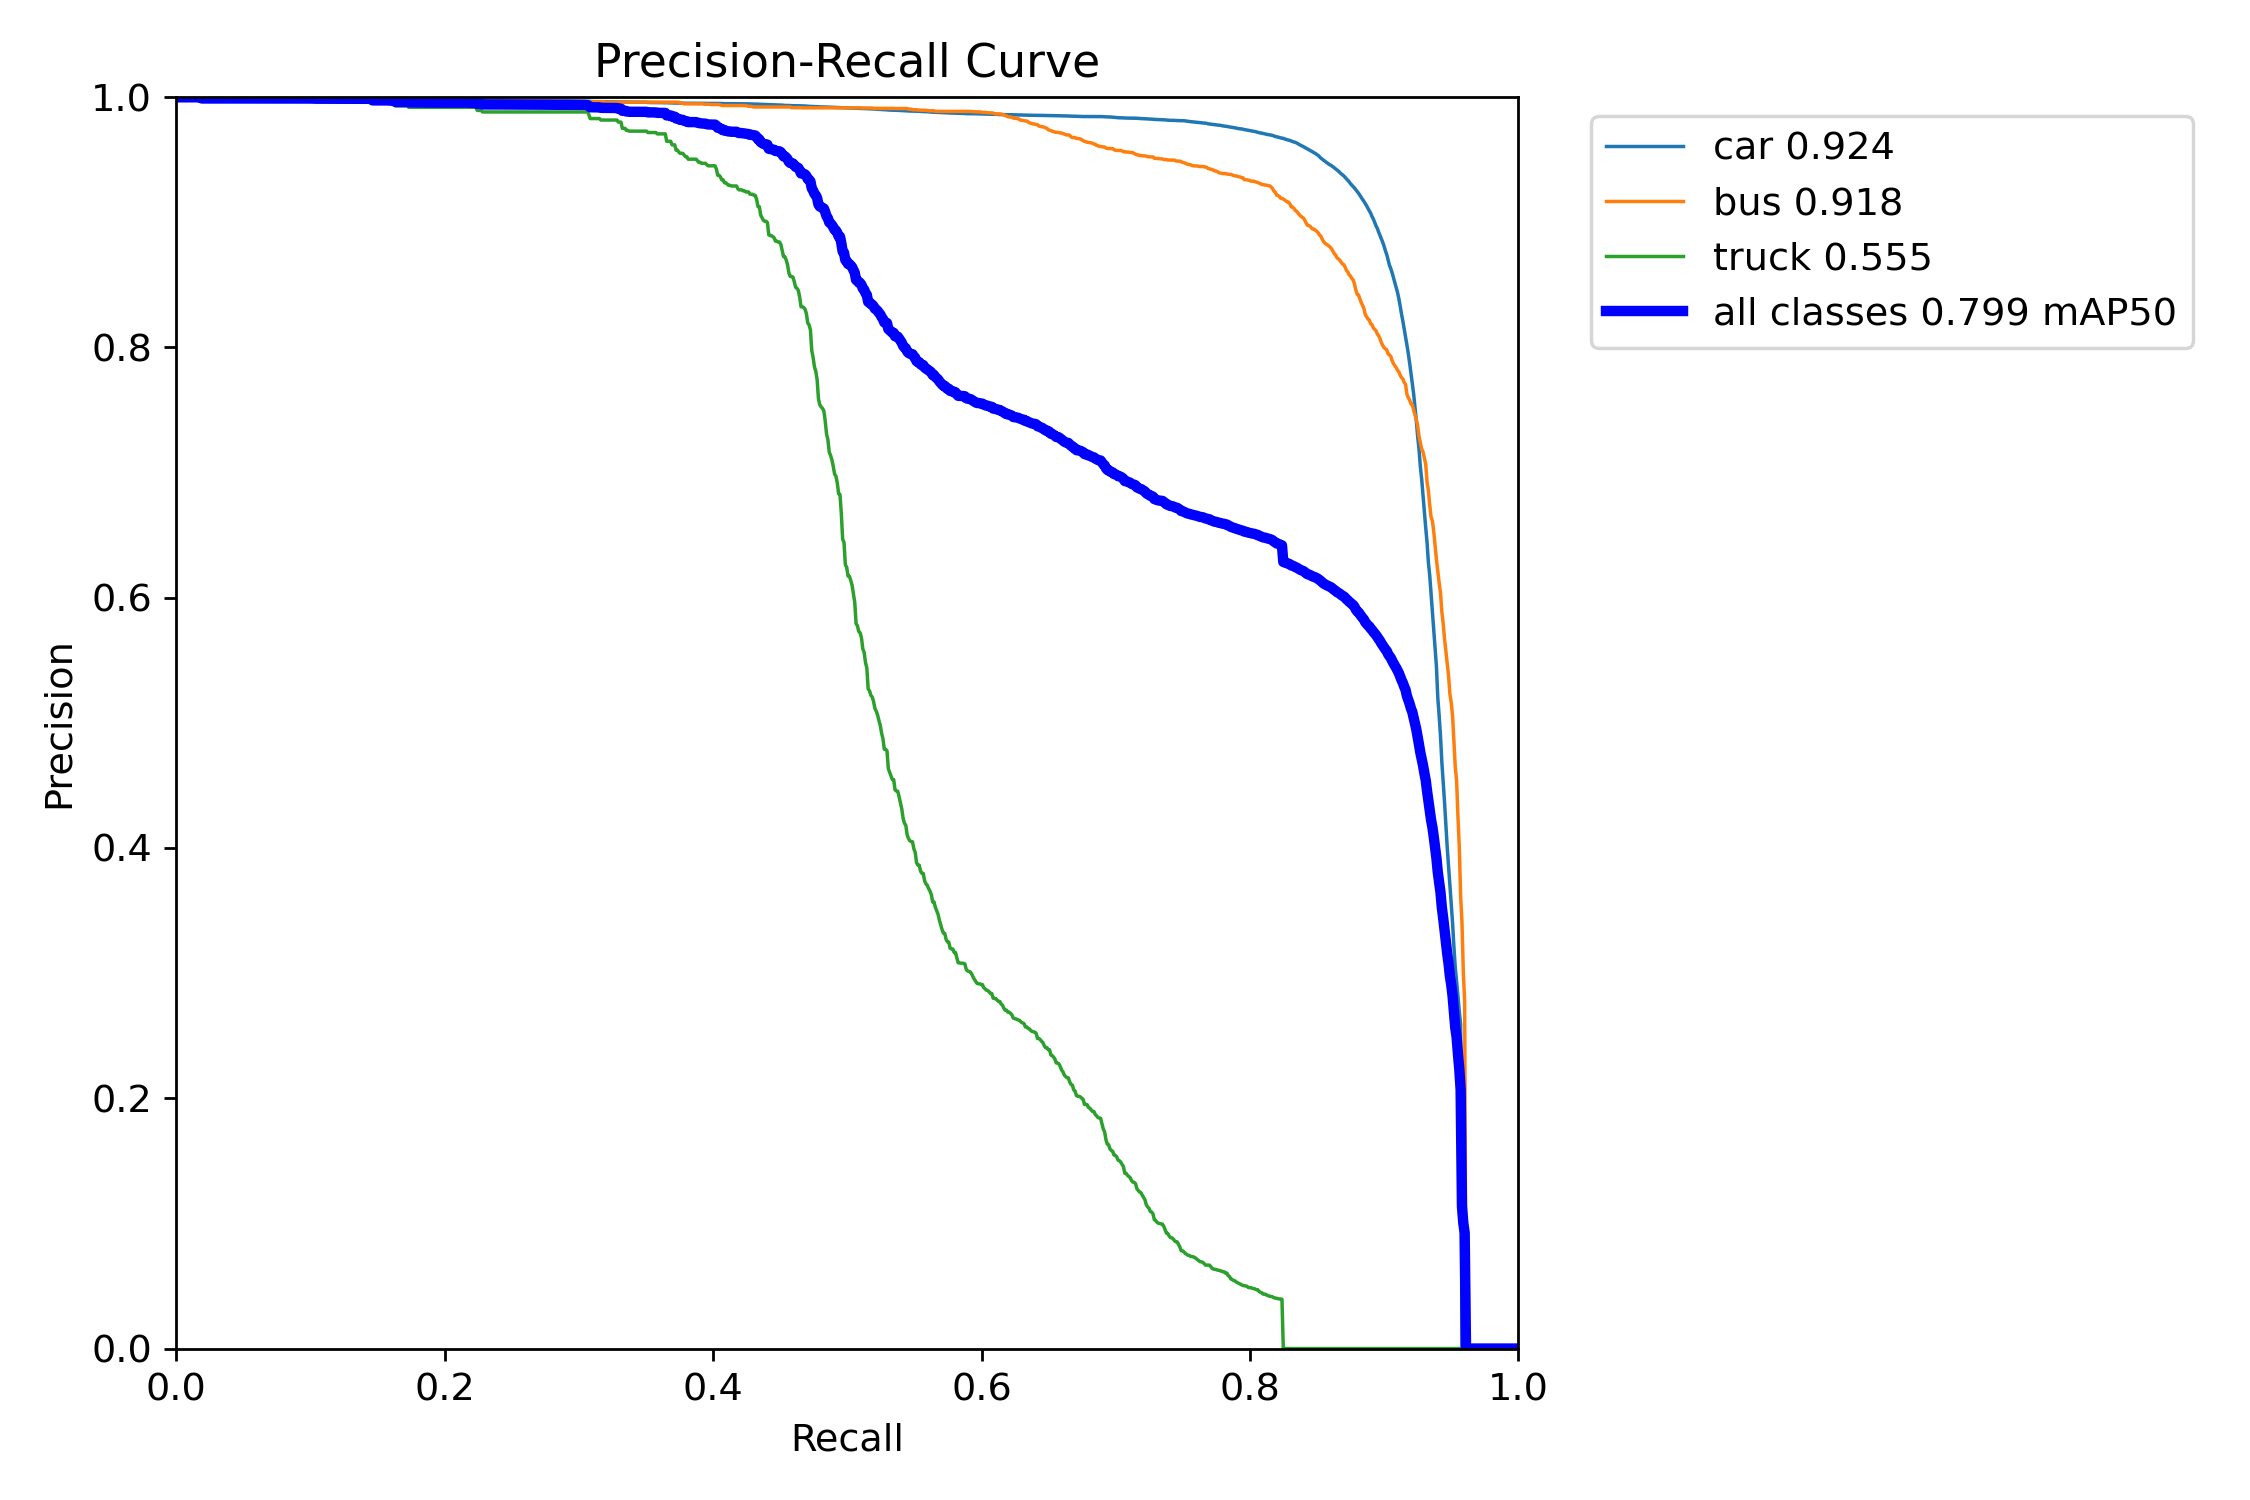
\includegraphics[width=0.75\textwidth]{figures/results/yolo_pr_curve.png}
\caption{Precision--recall curves of the fine-tuned detector on the UA-DETRAC test sequences}
\label{fig:yolo-pr}
\end{figure}

\section{Counting and Queue Estimation Results}

Table \ref{tab:counting} gives the count error of the complete detection, tracking, and line-counting chain over the 40 test sequences, where one sequence is one clip. Across all vehicles the mean absolute error is 2.60 vehicles per clip and the weighted absolute percentage error is 12.0 percent, with 11 of 40 clips counted exactly. Without the motorcycle class the error falls to 1.62 vehicles and 7.5 percent. Figure \ref{fig:count-scatter} plots the counted against the true number of crossings per clip.

\begin{table}[htbp]
\centering
\caption{Count error per clip on the 40 UA-DETRAC test sequences}
\label{tab:counting}
\begin{tabularx}{\textwidth}{Ycccccc}
\toprule
\textbf{Classes} & \textbf{True} & \textbf{Counted} & \textbf{MAE} & \textbf{Bias} & \textbf{WAPE} & \textbf{Exact clips}\\
\midrule
All vehicles & 870 & 972 & 2.60 & +2.55 & 12.0\,\% & 11\\
Car, bus, truck & 870 & 933 & 1.62 & +1.57 & 7.5\,\% & 15\\
Car & 800 & 852 & 1.35 & +1.30 & 6.8\,\% & 17\\
Bus & 61 & 77 & 0.40 & +0.40 & 26.2\,\% & 31\\
Truck & 9 & 4 & 0.17 & $-$0.12 & 77.8\,\% & 35\\
Motorcycle & 0 & 39 & 0.97 & +0.97 & -- & 31\\
\bottomrule
\end{tabularx}
\end{table}

\begin{figure}[htbp]
\centering
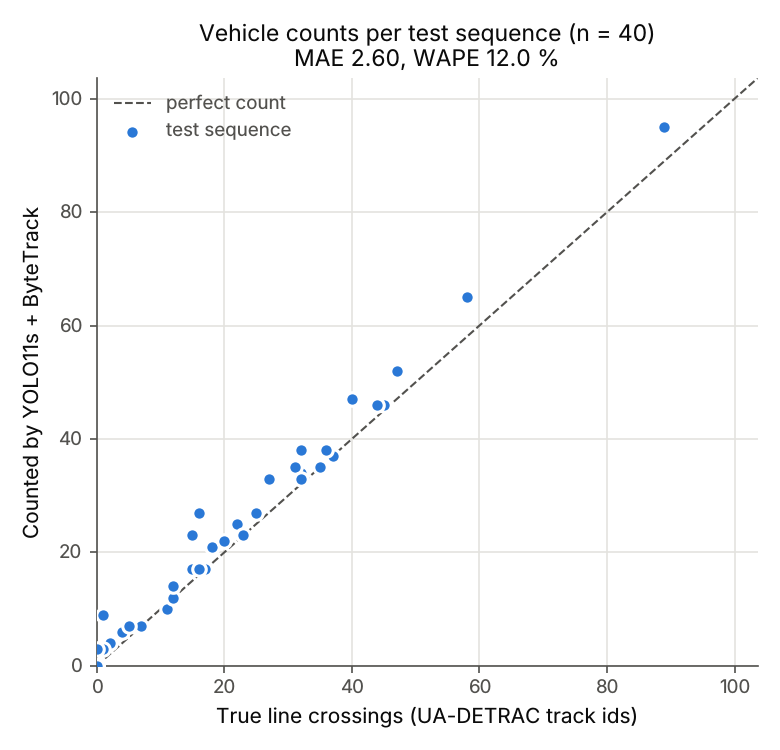
\includegraphics[width=0.55\textwidth]{figures/results/count_pred_vs_true.png}
\caption{Vehicles counted by the pipeline against true line crossings for each test sequence}
\label{fig:count-scatter}
\end{figure}

The error is almost entirely an over-count: no clip is under-counted by more than one vehicle. The likely causes are false detections, such as the stationary ``bus'' on the kerb island in Figure \ref{fig:queue-sample} (left), and identity switches near the line in dense traffic, which make one vehicle cross twice under two identities. This explanation comes from inspecting samples, not from a frame-by-frame audit. The 39 motorcycle counts cannot be judged with UA-DETRAC, which does not label two-wheelers; some may be real scooters or bicycles and some false detections. The queue proxy, the number of stopped tracked vehicles in view, has a mean per-frame absolute error of 0.80 vehicles. On the busiest clip, with about 30 stopped vehicles, the estimate follows the true value closely, as Figure \ref{fig:queue-sample} shows.

\begin{figure}[htbp]
\centering
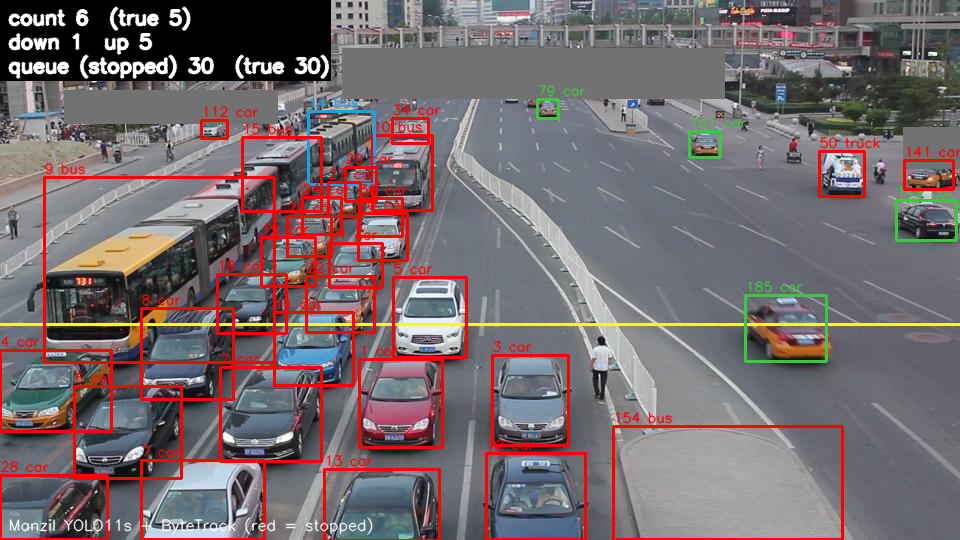
\includegraphics[width=0.48\textwidth]{figures/results/tracking_sample_frame.png}\hfill
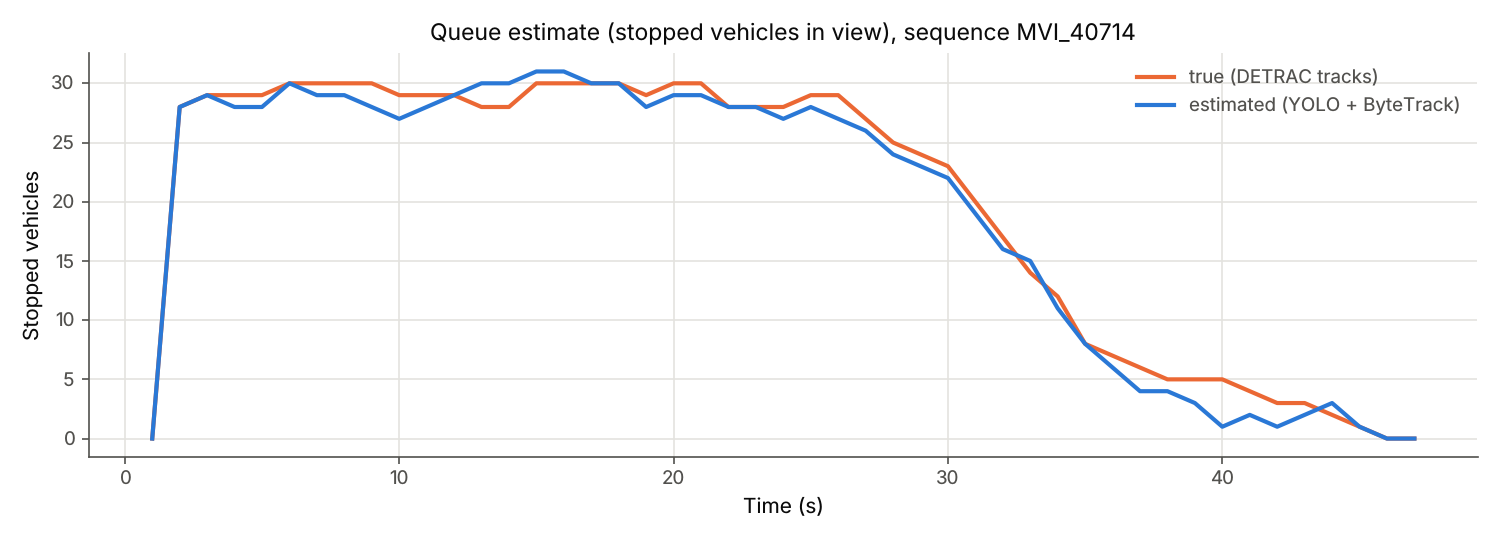
\includegraphics[width=0.48\textwidth]{figures/results/queue_sample.png}
\caption{Tracking with the counting line on test sequence MVI\_40714 (left) and estimated against true queue over the same sequence (right)}
\label{fig:queue-sample}
\end{figure}

\section{Signal Control Results}

Table \ref{tab:control-results} compares the three controllers on the four demand profiles, with tuned fixed-time control as the reference. Figure \ref{fig:control-comparison} shows the same data with the individual seeds.

\begin{longtable}{P{0.09\textwidth}P{0.16\textwidth}P{0.09\textwidth}P{0.10\textwidth}P{0.08\textwidth}P{0.27\textwidth}}
\caption{Signal-control results on the evaluation seeds (mean of 5 seeds)}\label{tab:control-results}\\
\toprule
\textbf{Profile} & \textbf{Metric} & \textbf{Fixed} & \textbf{Adaptive} & \textbf{DQN} & \textbf{DQN $-$ fixed (95\,\% CI), seeds better}\\
\midrule\endfirsthead
\caption[]{Signal-control results on the evaluation seeds (continued)}\\
\toprule
\textbf{Profile} & \textbf{Metric} & \textbf{Fixed} & \textbf{Adaptive} & \textbf{DQN} & \textbf{DQN $-$ fixed (95\,\% CI), seeds better}\\
\midrule\endhead
Light & Travel time (s) & 98.8 & 99.3 & 87.9 & $-$10.9 [$-$11.6, $-$10.2], 5/5\\
 & Waiting time (s) & 23.1 & 22.7 & 13.8 & $-$9.3 [$-$9.9, $-$8.8], 5/5\\
 & Max red (s) & 30.0 & 50.0 & 76.0 & +46.0 [43.2, 48.8], 0/5\\
\midrule
Medium & Travel time (s) & 109.0 & 104.3 & 98.6 & $-$10.4 [$-$10.6, $-$10.2], 5/5\\
 & Waiting time (s) & 30.3 & 23.9 & 20.1 & $-$10.2 [$-$10.5, $-$10.0], 5/5\\
 & Max red (s) & 35.0 & 50.0 & 62.0 & +27.0 [23.6, 30.4], 0/5\\
\midrule
Heavy & Travel time (s) & 172.9 & 175.7 & 155.7 & $-$17.2 [$-$23.4, $-$11.1], 5/5\\
 & Waiting time (s) & 75.9 & 67.8 & 57.4 & $-$18.5 [$-$22.4, $-$14.7], 5/5\\
 & Max red (s) & 55.0 & 50.0 & 73.8 & +18.8 [5.8, 31.8], 0/5\\
\midrule
Uneven & Travel time (s) & 118.5 & 121.6 & 108.0 & $-$10.5 [$-$11.8, $-$9.1], 5/5\\
 & Waiting time (s) & 37.3 & 34.9 & 26.1 & $-$11.2 [$-$12.2, $-$10.2], 5/5\\
 & Max red (s) & 55.0 & 50.0 & 74.8 & +19.8 [9.6, 30.0], 0/5\\
\bottomrule
\end{longtable}

\begin{figure}[htbp]
\centering
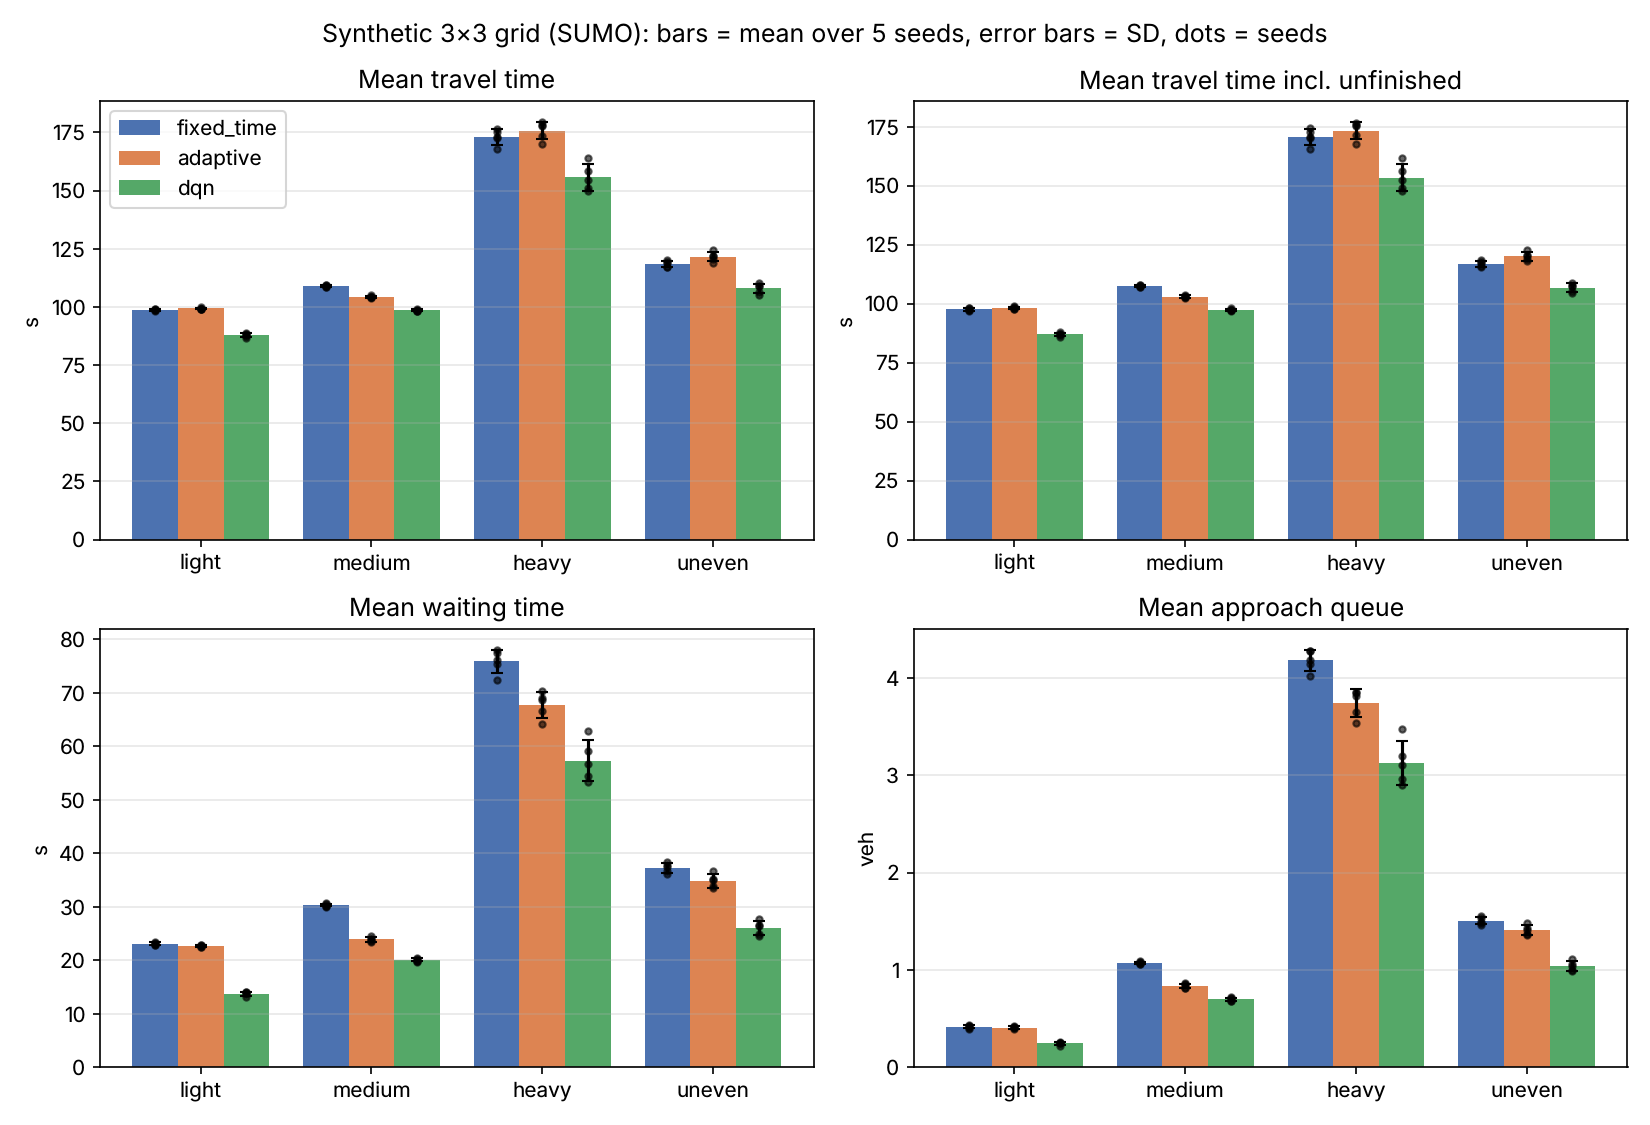
\includegraphics[width=\textwidth]{figures/results/controller_comparison.png}
\caption{Controller comparison on the synthetic grid: bars are means over five seeds, error bars standard deviations, and dots individual seeds}
\label{fig:control-comparison}
\end{figure}

The DQN reduced mean travel time against tuned fixed-time control by 11.0, 9.5, 10.0, and 8.9 percent on the light, medium, heavy, and uneven profiles, and mean waiting time by 24 to 40 percent, on every seed. The same reduction holds when unfinished vehicles are included (8.8 to 10.9 percent), so it is not caused by vehicles being stranded. Throughput was unchanged within 0.1 percent, except for a gain of 0.6 percent on heavy demand. The DQN also beat the adaptive controller on every travel-time and waiting-time comparison. Its cost is fairness: the longest time any phase waited rose from 30--55 s to 62--76 s on average, with a worst case of 89 s, just below the 90 s guard. The guard itself intervened 5 times in the 20 DQN runs.

The adaptive controller reduced waiting time on every profile, by 1.9 to 21.1 percent, and queues by 2 to 22 percent, but it reduced travel time only on medium demand ($-$4.3 percent). On light, heavy, and uneven demand travel time rose slightly, by up to 2.6 percent. The likely reason is more switching: on heavy demand it changed phase 1,535 times against 648 for fixed-time control, and each change costs 5 s of clearance. This explanation fits the data but was not tested separately. When the demand is not known in advance, represented by the single 35/35 s plan, the adaptive controller is clearly better on uneven demand, with a travel time of 121.6 s against 149.3 s and a waiting time of 34.9 s against 59.4 s.

\section{Emergency Routing Results}

In this experiment the corridor is off, and an obstruction that limits speed to 2 m/s starts at 1,000 s on road A1A2, which lies on the route that static routing chooses from free-flow costs. Static routing keeps that route; dynamic routing sees the reduced speed in its live costs and applies Algorithm \ref{alg:routing}. The measurement window was extended to 1,800 s because a first attempt with 900 s left four of five heavy-demand static trips unfinished; that attempt was discarded rather than reported without the failed trips.

\begin{table}[htbp]
\centering
\caption{Ambulance travel time with static and dynamic routing around an obstruction}
\label{tab:routing-results}
\begin{tabularx}{\textwidth}{p{0.14\textwidth}p{0.18\textwidth}p{0.18\textwidth}Yc}
\toprule
\textbf{Profile} & \textbf{Static (s)} & \textbf{Dynamic (s)} & \textbf{Difference (95\,\% CI)} & \textbf{Seeds better}\\
\midrule
Medium & 309.0 & 145.4 & $-$163.6 s [$-$201.7, $-$125.5], $-$53\,\% & 5/5\\
Heavy & 587.8 & 302.0 & $-$285.8 s [$-$408.6, $-$163.0], $-$49\,\% & 5/5\\
\bottomrule
\end{tabularx}
\end{table}

As Table \ref{tab:routing-results} shows, dynamic routing roughly halved the ambulance's travel time on both profiles and every seed. Ordinary traffic was not harmed: the network queue from dispatch until 300 s after arrival fell by 5.1 percent on medium demand (confidence interval crossing zero) and by 8.2 percent on heavy demand. All 20 ambulances arrived, and none crossed a red light. Figure \ref{fig:routing} shows the per-seed results.

\begin{figure}[htbp]
\centering
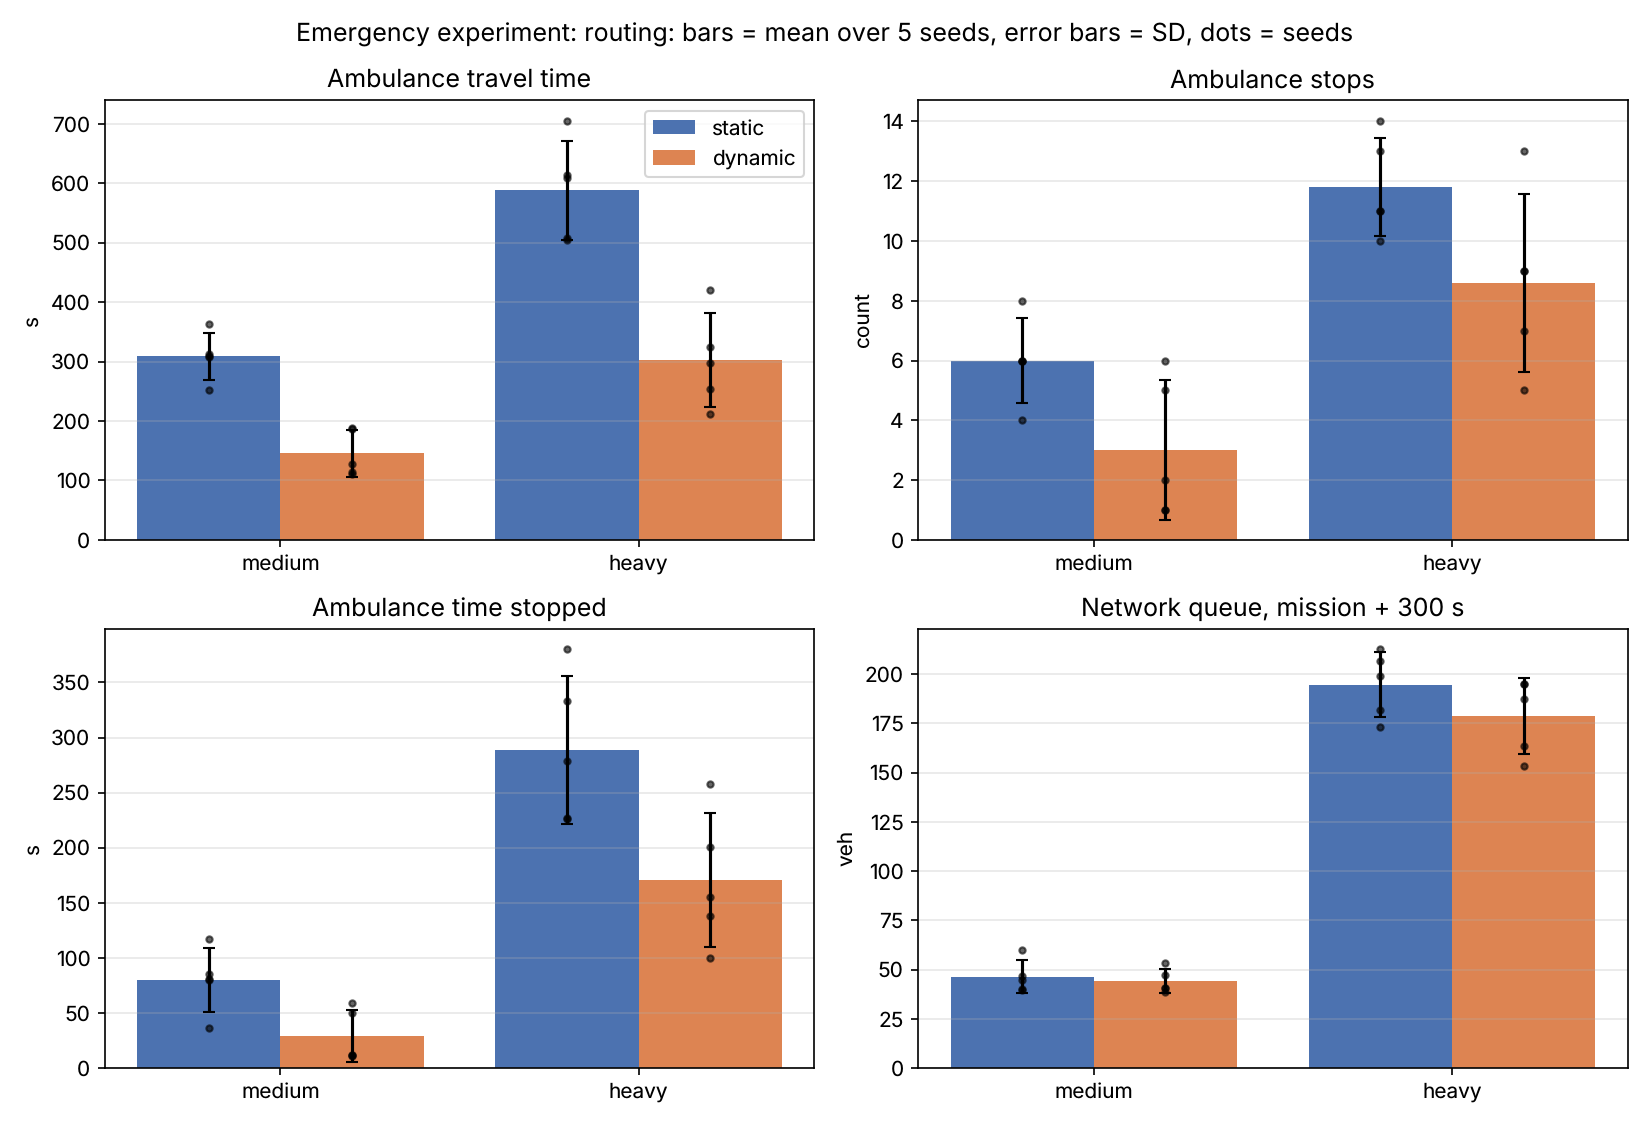
\includegraphics[width=0.9\textwidth]{figures/results/routing.png}
\caption{Static against dynamic routing around an obstruction}
\label{fig:routing}
\end{figure}

\section{Green Corridor Results}

The corridor experiment uses dynamic routing in both arms and no incident, so the difference comes from signal priority alone. Table \ref{tab:corridor-results} reports the corridor in its final form, with a 5 s corridor minimum green, against no corridor, with tuned fixed-time control for ordinary traffic.

\begin{table}[htbp]
\centering
\caption{Ambulance travel time and time stopped with the corridor off and on}
\label{tab:corridor-results}
\begin{tabularx}{\textwidth}{p{0.12\textwidth}p{0.16\textwidth}Yp{0.22\textwidth}}
\toprule
\textbf{Profile} & \textbf{Off $\rightarrow$ on (s)} & \textbf{Difference (95\,\% CI), seeds better} & \textbf{Time stopped (s)}\\
\midrule
Medium & 155.8 $\rightarrow$ 102.6 & $-$53.2 [$-$69.2, $-$37.2], $-$34\,\%, 5/5 & 45.2 $\rightarrow$ 4.4\\
Heavy & 313.6 $\rightarrow$ 127.8 & $-$185.8 [$-$278.5, $-$93.1], $-$59\,\%, 5/5 & 173.2 $\rightarrow$ 12.4\\
\bottomrule
\end{tabularx}
\end{table}

The corridor reduced the ambulance's travel time by 34 percent on medium and 59 percent on heavy demand, on every seed, and cut its time standing still by more than 90 percent. The cost to ordinary traffic was small: the network queue from dispatch until 300 s after arrival rose by 2.5 percent on medium and 3.0 percent on heavy demand, with both confidence intervals crossing zero, and mean waiting time over the window rose by 2.4 and 1.9 percent. A junction took on average 8.6 s (medium) and 13.8 s (heavy) to return to its usual queue after the ambulance passed. There were no safety violations, priority timeouts, or red-light crossings by the ambulance. Figure \ref{fig:corridor} shows the per-seed values.

\begin{figure}[htbp]
\centering
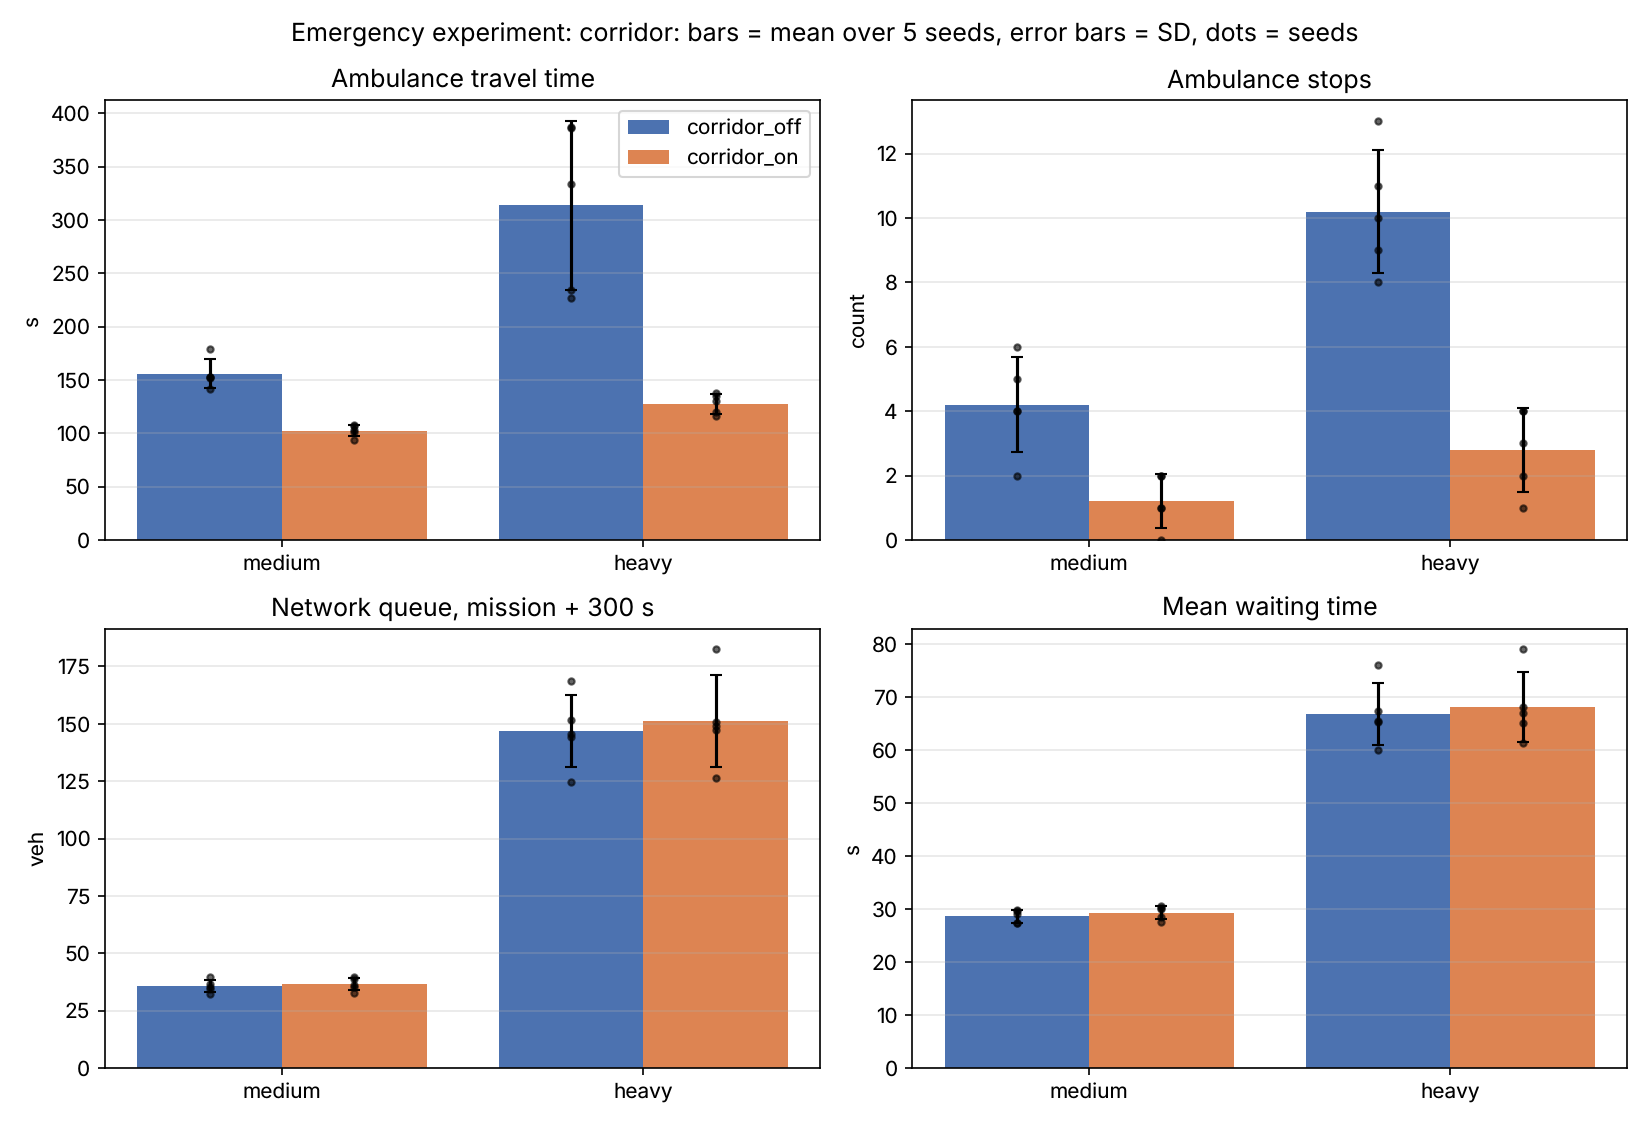
\includegraphics[width=0.9\textwidth]{figures/results/corridor.png}
\caption{Corridor off against on: ambulance travel time, stops, network queue, and waiting time}
\label{fig:corridor}
\end{figure}

Table \ref{tab:corridor-variants} summarizes the study of corridor variants described in Chapter \ref{ch:implementation}, which led to the 5 s corridor minimum green. With the route-index defect fixed (variant v1), the shortened green (v2) reduced the ambulance's travel time on heavy demand on four of five seeds with fixed-time control and on five of five with the DQN, while cross-street queueing changed by $-$3.7 to +2.4 percent. On medium demand the gain was negligible. Earlier activation gave gains of similar size that varied more between seeds, and raised cross-street queueing by 7 to 14 percent. The corridor also works with the DQN as background controller: with v2, the ambulance's travel time fell from 136.4 s to 101.0 s on medium and from 302.4 s to 124.2 s on heavy demand. Figure \ref{fig:stop-reasons} shows why the ambulance stood still in each variant: with the v1 and v2 corridors, all remaining stops are vehicles queued in front of it or waiting inside a junction, and none is at a red light.

\begin{table}[htbp]
\centering
\caption{Ambulance travel time for corridor variants (mean of 5 seeds; seeds better than v1 in brackets)}
\label{tab:corridor-variants}
\begin{tabularx}{\textwidth}{p{0.26\textwidth}YYYY}
\toprule
\textbf{Background and demand} & \textbf{Off (s)} & \textbf{v1 (s)} & \textbf{Earlier activation (s)} & \textbf{v2 (s)}\\
\midrule
Fixed-time, medium & 155.8 & 103.2 & 101.8 (2/5) & 102.6 (1/5)\\
Fixed-time, heavy & 313.6 & 136.0 & 134.0 (3/5) & 127.8 (4/5)\\
DQN, medium & 136.4 & 103.4 & 101.2 (4/5) & 101.0 (3/5)\\
DQN, heavy & 302.4 & 130.6 & 122.6 (3/5) & 124.2 (5/5)\\
\bottomrule
\end{tabularx}
\end{table}

\begin{figure}[htbp]
\centering
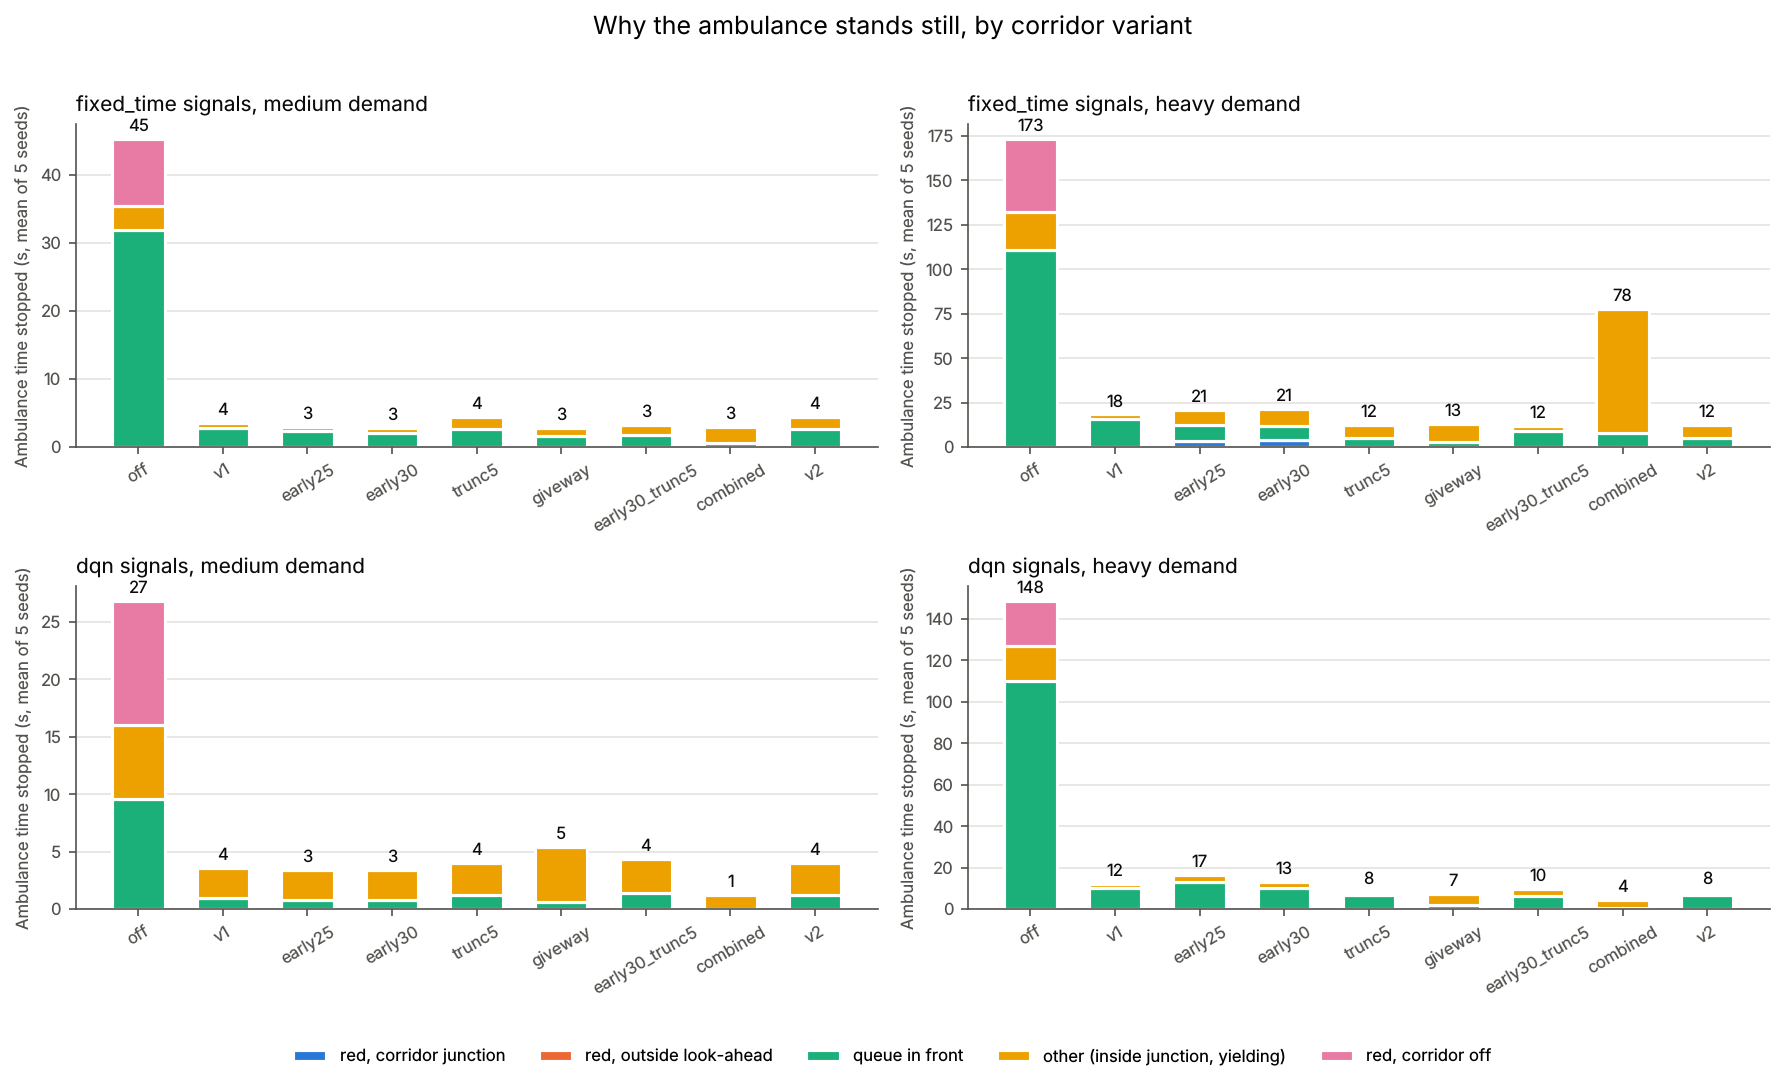
\includegraphics[width=\textwidth]{figures/results/corridor_stop_reasons.png}
\caption{Why the ambulance stood still, by corridor variant (mean seconds over five seeds)}
\label{fig:stop-reasons}
\end{figure}

One caution applies to these corridor numbers. The 5 s corridor minimum was chosen by comparing variants on seeds 0 to 4, the same seeds on which the corridor result is reported, so the v2 figures in Tables \ref{tab:corridor-results} and \ref{tab:corridor-variants} are development-stage estimates. The v1 corridor, which was designed before these runs, already reduced the ambulance's travel time by 34 percent on medium and 57 percent on heavy demand on the same seeds, so the main corridor effect does not depend on that choice. The v2 result will be confirmed on new seeds and on the Lahore network in FYP-II.

\section{Discussion}

The results support the main idea of the project within the tested conditions. A learned signal controller can reduce travel and waiting time compared with a well-tuned fixed plan, and live travel-time routing and a bounded corridor each give large reductions in ambulance delay, with small measured cost to ordinary traffic and no unsafe signal state in any run. The two emergency mechanisms are complementary: routing avoids a slow road, while the corridor removes waiting at signals on the chosen road. The perception chain counts vehicles with an error of about 12 percent per clip on public video, which is good enough to indicate demand but not yet good enough to replace simulator state in control experiments.

The results also show trade-offs that a single demonstration would hide. The DQN's gain comes partly from making minor phases wait longer, and only the safety filter's maximum-red guard keeps that wait bounded; a fairness term in the reward or a lower guard would cost some of the travel-time gain. The adaptive controller lowers waiting and queues but not total travel time against a tuned plan, which shows that a responsive rule is not automatically better than a good fixed plan. In perception, fine-tuning helped cars and buses but not trucks, which are rare in the training data, and could not improve motorcycles without local labels.

The main limits of the evidence are as follows. All simulation results come from one synthetic grid with one ambulance origin and destination, so they show behaviour on a controlled test track, not on Lahore roads. Five seeds were used instead of ten, and training and evaluation use the same four demand profile types on different seeds; there is no held-out demand pattern or second network yet. The DQN was trained once, so the variation between training runs is unknown. The corridor's downstream-capacity check and the compensation plan during recovery are not implemented, and the 5 s corridor result is a development-stage estimate as explained above. The detector has not been tested on Lahore video, which contains vehicle types and camera angles absent from UA-DETRAC. These limits define the FYP-II work in Chapter \ref{ch:conclusion}.

\section{Conclusion}

The FYP-I experiments produced measured, repeatable evidence for every main component of Manzil. The fine-tuned detector reached 0.799 mAP50 on UA-DETRAC test data, and the counting chain had a mean error of 2.60 vehicles per clip. On the synthetic grid the DQN reduced travel time by 9 to 11 percent against tuned fixed-time control at a cost in fairness to minor phases, dynamic routing roughly halved the ambulance's travel time around an obstruction, and the corridor reduced it by a further 34 to 59 percent with little cost to ordinary traffic. Each result is bounded by the network, data, and seeds on which it was measured, and the next chapter turns those bounds into the FYP-II plan.
